% Figure from MATH 591 notes, section 17. Compile with the notes preamble.
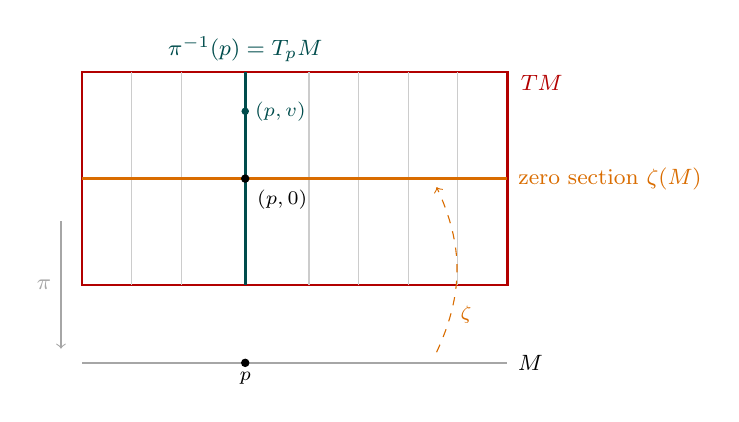
\begin{tikzpicture}[scale=0.9]
\draw[red!70!black, thick] (0,-1.5) rectangle (6,1.5); \node[red!70!black, font=\footnotesize, anchor=south west] at (6.05,1.1) {$TM$};
\draw[gray!40] (0.70,-1.5) -- (0.70,1.5);
\draw[gray!40] (1.40,-1.5) -- (1.40,1.5);
\draw[gray!40] (3.20,-1.5) -- (3.20,1.5);
\draw[gray!40] (3.90,-1.5) -- (3.90,1.5);
\draw[gray!40] (4.60,-1.5) -- (4.60,1.5);
\draw[gray!40] (5.30,-1.5) -- (5.30,1.5);
\draw[teal!60!black, very thick] (2.3,-1.5) -- (2.3,1.5) node[above, font=\footnotesize] {$\pi^{-1}(p) = T_pM$};
\draw[orange!85!black, very thick] (0,0) -- (6,0) node[right, font=\footnotesize] {zero section $\zeta(M)$};
\fill (2.3,0) circle (1.7pt); \node[font=\scriptsize, anchor=north west] at (2.33,-0.02) {$(p, 0)$};
\fill[teal!60!black] (2.3,0.95) circle (1.5pt) node[right, font=\scriptsize] {$(p, v)$};
\draw[thick, gray!70] (0,-2.6) -- (6,-2.6) node[right, font=\footnotesize, text=black] {$M$};
\fill (2.3,-2.6) circle (1.7pt) node[below, font=\scriptsize] {$p$};
\draw[->, gray!70] (-0.3,-0.6) -- node[left, font=\footnotesize] {$\pi$} (-0.3,-2.4);
\draw[->, dashed, orange!85!black] (5.0,-2.45) to[bend right=25] node[pos=0.22, right, font=\scriptsize] {$\zeta$} (5.0,-0.12);
\end{tikzpicture}
